%% Adaptive NMPC for Aerial Delivery Without Payload-Event Signals
%% ICRA manuscript; IEEE conference equation and figure conventions.
%% Build: latexmk -pdf main.tex   (or pdflatex x2 + bibtex)
%% Class: IEEEtran two-column conference; preserve template dimensions.
\documentclass[conference]{IEEEtran}
\IEEEoverridecommandlockouts

\usepackage{cite}
\usepackage{amsmath,amssymb,amsfonts}
\usepackage{graphicx}
\usepackage{booktabs}
\usepackage{multirow}
\usepackage{array}
\usepackage{siunitx}
\usepackage{xcolor}
\usepackage[hidelinks]{hyperref}
% State names remain upright small capitals even inside italic table notes.
\DeclareTextFontCommand{\textsc}{\upshape\scshape}

% Placeholder-figure helper: draws a framed box so the layout compiles before real figures exist.
\newcommand{\figplaceholder}[2]{%
  \fbox{\parbox[c][#2][c]{0.95\linewidth}{\centering\itshape #1}}}

\newcommand{\todo}[1]{\textcolor{red}{[TODO: #1]}}

\begin{document}

\title{Eventless Payload-Adaptive NMPC for Quadrotors}

% Double-anonymous review (ICRA 2027): author block withheld until acceptance.
\author{\IEEEauthorblockN{Anonymous Authors}
\IEEEauthorblockA{Affiliation withheld for double-anonymous review}}

\maketitle

\begin{abstract}
A release command does not guarantee that a payload has physically detached, so a controller
that clears its payload model on that command can fly a loaded vehicle as if it were empty. We
present an eventless payload-model interface for quadrotor nonlinear model predictive control
(NMPC) that never treats attach or release commands as evidence. A moving horizon estimator
(MHE) \cite{rao2003} estimates composite mass and the horizontal first mass moment
$s=m_P r_{xy}$ from odometry and a rotor-speed thrust proxy that is not computed from the
payload estimate; unlike a center-of-mass offset, $s$ remains well defined as the payload
vanishes. The inertia increment follows from the mass estimate and a weak vertical-arm prior,
and health-gated, rate-limited updates drive both the NMPC model and body-rate scheduling. In
PX4 \cite{px4} SITL with physically attached eccentric payloads, including a \SI{0.30}{kg},
\SI{4}{m/s} stress test at the vehicle's torque limit, release confirmation completed in 32 of
36 flights in which the payload attached and the vehicle survived to the release command; all
four failures, at \SI{4}{m/s}, trace to estimator failure. Confirmation took a median
\SI{3.46}{s} in maneuver and \SI{16.56}{s} after braking to hover. When detachment lagged the command by \SI{4}{s},
a baseline clearing on the command did so too early in 5/5 flights, but persistent confirmation,
with or without the command, never did; when no command reached the controller, the interface still detected
unsignaled payload loss in 10 of 18 flights. These results are limited to simulation
and the tested conditions.
\end{abstract}

\section{Introduction}
Autonomous aerial delivery and in-flight aerial manipulation subject a multirotor to abrupt
changes in its own dynamics. Grasping or releasing a parcel changes three coupled quantities
at once: the total \emph{mass} $m$ (which rescales the thrust-to-acceleration map and the
hover throttle), the \emph{center of mass} (a thrust that no longer passes through the
composite CoM produces a constant trim torque $\tau \approx \Delta r \times f$, significant
even for small offsets because $f \approx mg$ is large), and the \emph{rotational inertia}
(which slows the attitude response and effectively lowers the inner-loop bandwidth). The
first channel is an outer-loop (position/thrust) problem; the latter two are inner-loop
(attitude/rate) problems. A controller that models the payload only as a scalar mass will
mistrack or, for sufficiently heavy eccentric loads, destabilize.

\emph{Explicit parameter estimation} (EKF/MHE of mass, CoM, inertia) is interpretable and can
feed model-based constraints, but converges slowly across an abrupt change;
\emph{lumped-disturbance adaptation} (L1-adaptive NMPC, INDI) reacts fast but yields no physical
model; \emph{learning-based} estimators typically need rich sensing or ground-truth data.
We take the explicit route deliberately and accept its latency: the proposed interface trades
release-confirmation delay for semantics that never run ahead of physical evidence and for
named physical parameters.

The central question of this work is whether the complete grasp--carry--release lifecycle can
adapt its payload model without trusting a commanded or externally supplied payload event.
Our answer rests on two observations. First, payload mass and first moment can be estimated
continuously, with the inertia increment following algebraically from the mass estimate and a
weak geometric prior, without consuming a gripper command, attachment state, or external
event notification. Second, rotor-speed telemetry provides a collective-thrust and body-torque
proxy that is \emph{not computed from} the online payload estimate, under a calibrated rotor
thrust model; residuals formed from it therefore do not inherit a mass error through the
controller's own command. Combining the two, the estimator needs no external event signal and
no measurement of the horizontal attachment geometry.

\textbf{Contributions.}
\begin{enumerate}
\item A \textbf{first-moment payload interface}. Estimating mass together with the horizontal
first mass moment---the standard linear parameterization of rigid-body inertial parameters
\cite{atkeson1986}---keeps the payload geometry well defined through release, where a CoM
offset is not, and lets one health-gated $m/s/J$ frame drive bounded NMPC model updates and
continuous body-rate scheduling (\S\ref{sec:setup}--\ref{sec:method}).
\item \textbf{Release semantics that do not run ahead of evidence}: the controller clears its
payload model only after the estimator's no-payload confidence persists, never on its own
release command, and enters \textsc{unresolved} and brakes to hover when evidence is missing
(\S\ref{sec:method}).
\end{enumerate}
We evaluate the complete interface in PX4 SITL, reporting every attempt, the confirmation path
each flight took, a paired delayed-detachment fault injection, unsignaled partial payload loss,
and the failures observed at the vehicle's actuator limit (\S\ref{sec:autorelease},
\S\ref{sec:limits}).
The runtime estimator consumes only motor speeds and odometry; the sole geometric quantity not
identified online is a weak vertical-arm prior $r_z$, which is structurally unobservable from
the thrust-moment channel.

\section{Related Work}
\textbf{Agile quadrotor flight.} Geometric tracking on $\mathrm{SE}(3)$ \cite{lee2010} and
time-optimal flight \cite{foehn2021} assume known, fixed inertial parameters, which a payload
event invalidates mid-flight.

\textbf{Aerial manipulation and transport.} Aerial robots that grasp, carry and release
objects are surveyed in \cite{ollero2022}; dynamic aerial grasping, with explicitly modeled
gripper dynamics, was demonstrated in \cite{thomas2014}.
Load transportation, by grasping or cable suspension, is surveyed in \cite{villa2020}. Ours is
the transport-and-release subproblem: the payload is rigidly attached, so the controller must
handle the resulting change in mass, inertia and centre of mass.

\textbf{Control under changing payload.} Adaptive and robust designs---L1-adaptive NMPC
\cite{hanover2021}, INDI \cite{smeur}---treat the load as a lumped disturbance and are the
standard baselines for payload-carrying flight; L1-NMPC in particular reports large
tracking-error reductions under unknown load on aggressive trajectories. A parallel line
learns the residual dynamics instead: \cite{torrente2021} fits unmodeled aerodynamic effects
with Gaussian processes inside the MPC, which improves tracking without yielding a named
physical parameter either. Slung-load control
addresses the swinging-payload case explicitly \cite{sreenath2013}, exploiting differential
flatness of the cable-suspended system; a rigidly attached payload instead changes the
vehicle's own inertial parameters. A related proprioceptive line estimates the external wrench directly with momentum-based
observers, enabling collision detection and interaction control \cite{tomic2017}. All of these
recover a \emph{force/torque}, not a physical parameter: they cannot, e.g., update a
thrust-margin constraint or an inner-loop gain schedule from the estimate.

\textbf{MHE and online parameter estimation.} Filter- and optimization-based estimators
recover mass, inertia, and geometric parameters \cite{svacha2020,wuest2019,bohm2021}, and
the mass and CoM of a grasped payload have been estimated for aerial manipulation
\cite{mellinger2011}. Writing the CoM as a first mass moment makes inertial parameters enter the
dynamics linearly, a standard device in manipulator load identification \cite{atkeson1986}; we
use it because it remains well defined when the payload vanishes.
Standard MHE performance is highly sensitive to the process/measurement weight matrices;
neural MHE (NeuroMHE) \cite{neuromhe} learns to output these weights online, resolving the
bias--variance trade-off but estimating a lumped disturbance force rather than explicit named
parameters.

\textbf{Residual-based change detection.} Residual-based fault/change detection (CUSUM and
related methods \cite{basseville1993}) motivates the evidence checks used by the payload
lifecycle state machine. Our positioning: we do not learn dynamics and add no sensing; every
deployed signal derives from motor speeds and odometry. This is a deliberate
departure from learning-based MPC \cite{hewing} and the broader safe-learning agenda
\cite{brunke}, where a learned component absorbs the model mismatch; here the mismatch is
resolved into named parameters that downstream constraints can consume.

\section{System Overview and Problem Setup}\label{sec:setup}
\textbf{Architecture (Fig.~\ref{fig:arch}).} Three layers: Gazebo physics (with a magnetic
DetachableJoint gripper producing genuine inertia/CoM changes), the PX4 inner-loop rate
controller, and a ROS~2 outer loop (NMPC + MHE). The outer loop publishes a collective thrust
and a body-rate setpoint; PX4 tracks the body rate.

\begin{figure*}[t]
\centering
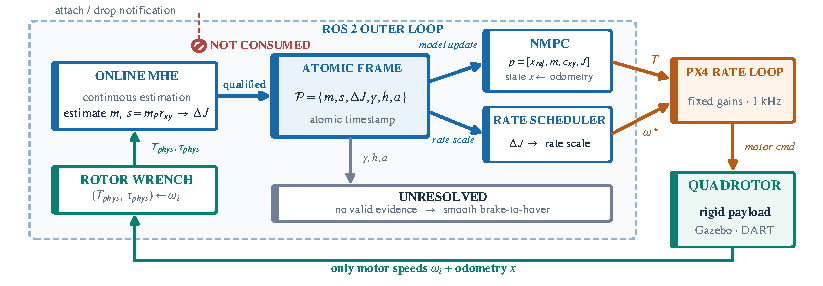
\includegraphics[width=0.95\textwidth]{figs/fig1_architecture.pdf}
\caption{System architecture and information flow. The full pipeline consumes only motor
speeds and odometry; one atomic, health-gated $m/s/J$ frame drives both the NMPC model and
continuous rate-command scheduling. No attach/drop notification enters this path.}
\label{fig:arch}
\end{figure*}

\textbf{Dynamics and parameterization.} The NMPC model carries the runtime parameter vector
$p = [x_{\text{ref}}, m, \Delta J, c_{xy}]$ (extended with a lumped disturbance only for the
L1 baseline). Thrust acting at the geometric center about the composite CoM produces
$\tau_{\text{com}} = [-c_y T, +c_x T, 0]$. The NMPC solves
\begin{equation}
\begin{aligned}
\min_{u_{0:N-1}}\;& \textstyle\sum_{k=0}^{N-1}\bigl(\lVert e_k\rVert_{Q}^2
  +\lVert u_k-\bar u(p)\rVert_{R}^2\bigr)+\lVert e_N\rVert_{Q_N}^2\\
\text{s.t.}\;& x_{k+1}=F(x_k,u_k,p),\quad x_0=\hat x,\quad u_k\in\mathcal U,
\end{aligned}
\label{eq:nmpc}
\end{equation}
where $x\in\mathbb R^{13}$ stacks position, velocity, attitude quaternion and body rate,
$u=[T,\tau^{\mathsf T}]^{\mathsf T}$, $e_k$ stacks the position, velocity, quaternion-vector and
rate errors to the reference, and $F$ is one RK4 step ($\Delta t=\SI{0.05}{s}$, $N=20$). The
input reference $\bar u(p)=[mg,\,c_y mg,\,-c_x mg,\,0]^{\mathsf T}$ is the live hover input
including the eccentric trim torque. $Q$ and $R$ follow Bryson's rule with tolerances
\SI{0.1}{m}, \SI{0.3}{m/s}, 0.05, \SI{0.3}{rad/s}, \SI{2}{N} and the torque bounds; $Q_N$
scales the position, attitude and rate blocks of $Q$ by 20, 2 and 0.2. $\mathcal U$ is the
actuator envelope $T\in[1.27,31.35]$\,N, $|\tau_x|,|\tau_y|\le\SI{0.5}{N\,m}$,
$|\tau_z|\le\SI{0.2}{N\,m}$. The deployed MHE augments both composite mass and
the horizontal first mass moment,
\begin{equation}
\begin{aligned}
x_{\mathrm{MHE}} &= \begin{bmatrix}x^{\mathsf T} & m & s_x & s_y\end{bmatrix}^{\mathsf T}
                   \in\mathbb{R}^{16},\\
s &= m_P r_{xy},
\end{aligned}
\label{eq:mhe-state}
\end{equation}
with $\dot m=0$ and $\dot s=0$ within each window ($N=20$, $\Delta t=\SI{0.1}{s}$). It solves
\begin{equation}
\begin{aligned}
\min_{x,\,w}\;& \lVert x_0-\bar x_0\rVert_{W_0}^2\\
& {}+\textstyle\sum_{j=0}^{N-1}\beta_j\bigl(\lVert y_j-Cx_j\rVert_{W_y}^2
  +\lVert w_j\rVert_{W_w}^2\bigr)\\
\text{s.t.}\;& x_{j+1}=F_{\mathrm M}(x_j,u^{\mathrm{phys}}_j)+Gw_j,\\
& m\in[0.95\,m_B,\,\SI{5}{kg}],\quad |s_x|,|s_y|\le\SI{1.5}{kg\,m},
\end{aligned}
\label{eq:mhe}
\end{equation}
over $x_{0:N}$ and $w_{0:N-1}$, where $y_j$ is the odometry and $C$ selects the 13 vehicle
states,
$u^{\mathrm{phys}}=[T_{\text{phys}},\tau_{\text{phys}}^{\mathsf T}]^{\mathsf T}$ is reconstructed
from rotor speeds (below), and $G=[I_{13},0]^{\mathsf T}$ keeps $m$ and $s$ noise-free.
$W_y$ is the inverse squared odometry noise (\SI{0.02}{m}, \SI{0.05}{m/s}, 0.01,
\SI{0.02}{rad/s}); $W_w=\mathrm{diag}(10^4 I_6,10^5 I_4,10^3 I_3)$ deliberately trusts the
dynamics. The arrival cost $W_0=\mathrm{diag}(10^3 I_6,10^4 I_4,10^2 I_3,0.1,100\,I_2)$ is
centred on the previous window's shifted solution and is nearly uninformative in $m$
($\sigma\approx\SI{3.2}{kg}$) and $s$ ($\sigma=\SI{0.1}{kg\,m}$). In the reported \SI{4}{m/s} conditions $\beta_j\equiv1$. An earlier residual-triggered
schedule, which scaled stages preceding a self-detected $T_{\text{phys}}$ step (\SI{4.4}{N} from
a slow baseline) by $10^{-4}$, remained armed in the \SI{2}{m/s} flights but never fired there; it was
disabled at \SI{4}{m/s} because grasp and release transients crossed its threshold. No external
event enters $\beta_j$. The published geometry is reconstructed as
\begin{equation}
\begin{aligned}
c_{xy} &= \frac{s}{m},\\
\mu &= \frac{m_B\max\{m-m_B,0\}}{m},\\
\Delta J_{xx} &= \Delta J_{yy}=\mu r_z^2,
\end{aligned}
\label{eq:continuous-geometry}
\end{equation}
where $r_z$ is a weak prior from the payload rack. The small $O(r_{xy}^2)$ diagonal terms and yaw increment are
omitted in the deployed interface.

\textbf{Estimate-independent thrust proxy.} We reconstruct the collective thrust
$T_{\text{phys}} = k \sum_i \omega_i^2$ and the body torques from rotor speeds and arm
geometry. The quadratic coefficient $k$ is a static-thrust constant; it is known to lose
validity under large induced inflow during fast translation \cite{bangura2012}, which we do
not model. Feeding the NMPC's \emph{commanded} thrust back into the estimator would instead
close an estimator--controller loop: that command is computed from $\hat m$ itself (its cost
anchors $T$ near $\hat m g$), and any inversion error, saturation, or motor lag between command
and rotor is invisible to the estimator, so a mass error can persist self-consistently rather
than appear as a residual. The rotor-speed proxy is taken downstream of those stages and is not
computed from $\hat m$; it does depend on the calibrated $k$, and in our simulator the plant
generates thrust with the same square law (\S\ref{sec:limits}).

\textbf{Thrust-to-throttle inversion.} The offboard collective-thrust command is inverted to a
normalized rotor command through the motor model $T = k\omega^2$. Provided that the forward
thrust reconstruction and inverse command mapping use the same $k$, steady-state closed-loop
tracking is generally not directly affected by its absolute value.

\textbf{Continuous inner-loop scheduling.} Model consistency in the NMPC cannot by itself
restore the PX4 rate loop's lost bandwidth. The deployed path therefore maps the live inertia
increment to a body-rate-command scale, low-pass filters it, applies target hysteresis and
asymmetric rise/recovery slew limits, and preserves \SI{5}{\percent} command headroom before
the final saturation. It does \emph{not} rewrite PX4 parameters. An attach-time inertia-only
bootstrap uses the rack's \SI{0.30}{kg} maximum payload for immediate safety, then fades out
after persistent coherent MHE evidence; neither payload mass nor $s$ is injected by this
bootstrap, and the drop path remains estimate-only.

\section{Online Estimation and Eventless Adaptation}\label{sec:method}
\subsection{Continuous payload interface and autonomous lifecycle}
The MHE publishes one atomic frame
\begin{equation}
\begin{aligned}
\mathcal{P}=\bigl\{&m,s_x,s_y,c_x,c_y,\\
                 &\Delta J_{xx},\Delta J_{yy},\Delta J_{zz},\\
                 &J_{xx},J_{yy},J_{zz},\gamma,h,a\bigr\},
\end{aligned}
\label{eq:payload-frame}
\end{equation}
where $\gamma$ is no-payload confidence, $h$ is a health bit and $a$ is solution age. Health
requires a successful latest solve and fresh odometry, motor-speed, and known-input streams.
The NMPC additionally checks local receive age; an unhealthy or stale frame freezes the last
accepted model and breaks the confidence persistence timer. Valid frames pass through a
low-pass filter and separate slew limits for $m$, $s$, and $\Delta J$ before every NMPC solve.

Payload presence is an estimator-owned state, distinct from any externally signalled attach
state. A hysteretic \textsc{empty}$\leftrightarrow$
\textsc{loaded} machine uses sustained payload-mass evidence, with a directional residual as a
fast path, and a separate latch records that the present flight reliably entered
\textsc{loaded}. This latch prevents an empty-flight confidence value from consuming the later
drop confirmation and prevents a transient mass dip during a figure-eight from disarming the
true release path.

No-payload confidence is the product of smooth empty scores for payload quantity, first moment,
and inertia. A nonzero moment therefore vetoes a false empty decision even if the mass estimate
touches its lower bound. On accepted release evidence, the estimator switches only the
\emph{published target} of $s$ to zero; the optimization state is not overwritten. The output
filter consequently produces a continuous decay rather than a geometric step. The controller
marks a planned drop complete, resets its L1 state, and finishes recovery only after healthy
confidence remains above 0.90 for \SI{1.0}{s}; issuing the gripper command itself does none of
these things.

\subsection{Why the first mass moment is the essential state}
Estimating CoM offset alone is ill-conditioned at release: physically
$s=m_P r_{xy}\rightarrow0$, whereas $r_{xy}$ itself is undefined as $m_P\rightarrow0$. In an
earlier mass-only formulation, the optimizer could suppress a phantom eccentricity only by
driving total mass below the bare-airframe value; 14 of 55 post-release samples then pinned at
the lower bound. Augmenting $s$ supplies the rotational channel directly and permits
$c_{xy}=s/m$ without knowing the grasp-dependent horizontal offset. A frozen-window inertia
coefficient prevents the optimizer from using instantaneous mass as a free inertia knob, while
the weak $r_z$ prior retains the dominant parallel-axis term. It is the smallest structure we
found that represents payload existence, trim moment, and roll/pitch inertia without an
external attachment geometry measurement.

\textbf{Estimator declaration and controller confirmation.} The controller clears its payload
model through one route only: confirmation, i.e.\ $\gamma>0.90$ held for \SI{1.0}{s} on healthy,
fresh frames. The estimator may additionally \emph{declare} release, which switches the
published target of $s$ to zero and so speeds the rise of $\gamma$; a declaration is neither
necessary nor sufficient for confirmation. The final code has two declaration routes.
(a)~A \emph{moment-gated detector} requires collapse of
$\rho=\lVert s\rVert/\lVert s\rVert_{\mathrm{ref}}$ below 0.30, where the loaded reference is
formed from a healthy, low-dynamic, in-envelope interval and frozen before aggressive flight. It
fires on quantity-empty plus moment-collapse evidence for five frames (slow path), or on moment
collapse accompanied by a persistent signed thrust-residual step
$\Delta T=\overline{T}_{\mathrm{post}}-\overline{T}_{\mathrm{pre}}$ over \SI{0.3}{s}
half-windows (moment--residual path). (b)~A \emph{mass-domain route} declares release after
$m_P<\SI{0.030}{kg}$ for 20 frames, accumulated only in low-dynamic flight. Confirmation can
also occur without any declaration; because the confidence's moment score uses an absolute
bound on $\lVert s\rVert$, a nonzero moment still vetoes it. Neither (b) nor confidence alone
uses the frozen-reference ratio, so confirmations through them are not evidence for (a);
Sec.~\ref{sec:autorelease} reports how often each occurred. Moment evidence must come from a
fresh, successful solve: re-anchoring after five consecutive solver failures initializes $s$
to zero, and that value is not counted as collapse. During development we also tested a
quantity--residual branch (a \SI{0.9}{N} residual plus quantity-empty evidence, without moment
evidence); it was removed after premature releases (Sec.~\ref{sec:autorelease}). A recorded
figure-eight transient reached \SI{-1.69}{N}, larger in magnitude than the \SI{-1.47}{N} step of
the smallest payload, so residual amplitude alone cannot separate the cases. Online and offline
evaluation call the same pure decision function, and an \textsc{unresolved} timeout is treated
as unknown, never as proof of an empty vehicle.

Table~\ref{tab:thresholds} lists the lifecycle thresholds and where each value comes from. All
were fixed in code before the final campaign began and were not retuned on it. Only $\rho$ and
the residual floor were selected against data from earlier flights; the remaining values are
engineering choices whose closed-loop sensitivity we have not swept.

\begin{table}[tb]
\caption{Lifecycle thresholds and their provenance. ``Earlier flights'' predate, and are
disjoint from, the reported campaign.}
\label{tab:thresholds}
\centering
\scriptsize
\setlength{\tabcolsep}{3pt}
\begin{tabular}{@{}>{\raggedright\arraybackslash}p{0.25\linewidth}>{\raggedright\arraybackslash}p{0.22\linewidth}>{\raggedright\arraybackslash}p{0.47\linewidth}@{}}
\toprule
threshold & value & provenance \\
\midrule
moment-collapse ratio $\rho$ & 0.30 & leave-one-out cross-validation on 59 earlier flights; every fold chose 0.30 (0.20 succeeded in 48/59) \\
residual floor / persistence & \SI{0.9}{N}; 2 or 4 frames & below the \SI{1.47}{N} weight of the smallest payload; on a recorded flight, figure-eight excursions above \SI{0.9}{N} lasted $\le3$ frames, the release step 4 frames \\
slow-path persistence & 5 frames (\SI{0.5}{s}) & engineering choice \\
mass-domain release & $m_P<\SI{0.030}{kg}$, 20 frames & between the loaded minimum (\SI{0.079}{kg}) and post-release maximum (\SI{0.007}{kg}) of earlier \SI{0.15}{kg} flights \\
no-payload confidence & 0.90 for \SI{1.0}{s} & engineering choice \\
\textsc{unresolved} timeout / brake & \SI{12}{s} / \SI{3}{s} & engineering choice \\
\bottomrule
\end{tabular}
\end{table}

\section{Simulation Setup}\label{sec:sim}
PX4 SITL with Gazebo \cite{gazebo} (Harmonic), an x500 quadrotor, and a magnetic DetachableJoint gripper
that produces genuine inertia and CoM changes.

The physical DetachableJoint gripper attaches a separate rigid body and therefore couples
mass, inertia and CoM together. It supports the lifecycle, baseline, and safety claims in the
paper; no wrench-emulated mass-step result is retained.

Task sequence (Fig.~\ref{fig:track3d}): approach (position control)
$\rightarrow$ NMPC hand-off and warmup hover $\rightarrow$ controlled descent $\rightarrow$
active grasp enable $\rightarrow$ lift $\rightarrow$ figure-eight $\rightarrow$
phase-triggered release. We state the NMPC scope explicitly: it governs the grasp hover and
the post-event adaptation phase; the approach controller is not part of the claim.
Batches run headless, with a stand-in process supplying the ground-station heartbeat that PX4
requires.

\begin{figure}[tb]
\centering
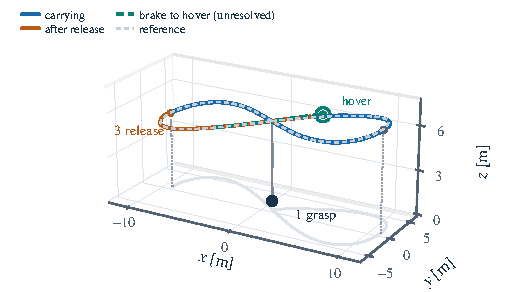
\includegraphics[width=\linewidth]{figs/fig_track_3d_measured.pdf}
\caption{Measured mission trajectory (simulator ground truth), two \SI{0.15}{kg}/\SI{2}{m/s}
flights of the same batch: grasp (1), lift, then carry along the figure-eight with \SI{\pm0.8}{m} vertical undulation (blue)
against the nominal reference (pale dashed). After the release command (3) one flight clears the
moment vote in maneuver and keeps tracking (orange); the other declares \textsc{unresolved} at
its \SI{12}{s} timeout and brakes to a hover (teal), confirming at \SI{16.40}{s}. The two paths
agree to within \SI{0.12}{m} (median) before the timeout; loaded tracking RMS is \SI{0.053}{m},
and \SI{0.060}{m} after release.}
\label{fig:track3d}
\end{figure}

\emph{Real-time budget.} Both optimizers are acados \cite{acados} SQP solvers with merit
backtracking and the HPIPM \cite{hpipm} QP solver. On one desktop core shared with Gazebo/PX4
SITL, the deployed 13-state NMPC ($N=20$, \SI{20}{Hz}) solves in \SI{1.3}{ms} at the median and
\SI{2.2}{ms} at the 99th percentile ($n=1009$), i.e.\ \SI{2.6}{\percent} and \SI{4.4}{\percent}
of its \SI{50}{ms} period. The deployed 16-state first-moment MHE ($N=20$, \SI{10}{Hz}) solves
in \SI{9.2}{ms} at the median, \SI{24.6}{ms} at the 90th and \SI{59.2}{ms} at the 99th
percentile, with a \SI{72.8}{ms} maximum ($n=\num{3740}$, first 20 frames per flight discarded),
against a \SI{100}{ms} period---roughly $7\times$ the \SI{1.4}{ms} median of the historical
mass-only estimator. This meets the deadline in simulation, but the tail margin is narrow, so we
make \emph{no} onboard-headroom claim; that requires measurement on the target computer.
Setpoints are published at \SI{50}{Hz} by interpolating the latest prediction.

\section{Results}\label{sec:results}
\emph{Provenance.} The lifecycle cohort uses the final 16-state first-moment interface; its
two \SI{4}{m/s} conditions were re-flown with the residual-triggered schedule disabled, and all
lifecycle flights predate the window-based re-initialization seed of \S\ref{sec:limits}.
The baseline matrix was recorded with the earlier mass-only 14-state MHE and supports only
the bounded baseline comparison stated below; it does not evaluate the proposed first-moment
interface. In Table~\ref{tab:matrix}, \emph{truth}
gives the NMPC the attachment geometry measured in simulation, \emph{online} replaces the CoM
offset with a motor-torque-inversion estimate, and \emph{l1} is the L1-adaptive baseline.

\iffalse
The following detailed CEM and precursor-geometry development record is retained in the source
for supplementary use but excluded from the focused manuscript.
\subsection{Learned weight scheduling: a negative result}
We pre-register \textbf{settling time} as the primary metric and report \textbf{within-run
paired differences}, never cross-batch absolutes---the M0 baseline itself moves by \SI{0.9}{s}
across sessions and solver configurations, larger than the effect under test.

Neither search yields a transferable gain, and the two fail differently. The absolute-threshold
search descends monotonically in training ($11.05 \rightarrow 9.74$, $-12\%$) yet lands
\emph{level with} M0 on a cell held out in both axes; the $\alpha$-parameterized search does not
descend at all ($10.46 \rightarrow 10.67$) yet wins 6/6 paired repetitions on that same cell.
A descending training curve and a small held-out win are thus each, on their own, uninformative
here.

We therefore test the surviving candidate $\theta^\star$ against M0 in a pre-registered
$2\times2$ factorial separating its two differences---the dimensionless threshold $\alpha$ and
the four rhythm dimensions, which are orthogonal in the implementation. Arms run back-to-back
within each repetition with order rotated by a 4-order Latin square; $n=8$ per cell, geometry
prior at truth, 64 runs, zero divergence.

\begin{table}[tb]
\caption{Paired median differences vs.\ M0 (primary metric: settling; negative favors the
learned schedule; exact Wilcoxon signed-rank).}
\label{tab:learn}
\centering
\begin{tabular}{@{}lcc@{}}
\toprule
contrast & \SI{0.2}{kg} & \SI{0.3}{kg} \\
\midrule
M0 $\rightarrow$ $\alpha$-only & $+0.20$ ($p=.25$) & $+0.15$ ($p=.20$) \\
rhythm-only $\rightarrow$ $\theta^\star$ & $+0.05$ ($p=.74$) & $-0.35$ ($p=.055$) \\
M0 $\rightarrow$ rhythm-only & $+0.00$ ($p=.84$) & $+0.30$ ($p=.25$) \\
$\alpha$-only $\rightarrow$ $\theta^\star$ & $-0.20$ ($p=.25$) & $-0.15$ ($p=.078$) \\
\midrule
\textbf{M0 $\rightarrow \theta^\star$ (total)} & $\mathbf{-0.05}$ ($p=.95$) &
$\mathbf{+0.00}$ ($p=.84$) \\
\bottomrule
\end{tabular}
\end{table}

All ten settling-time tests are non-significant (smallest $p=.055$) and the total effect is a
median of zero at both masses: \textbf{neither factor contributes a measurable gain}. This is
not a power problem---against the effect sizes previously attributed to $\theta^\star$
($-0.64$, $\SI{-0.40}{s}$) and the paired standard deviations measured here (0.407,
\SI{0.311}{s}), Cohen's $d_z$ is 1.57 and 1.29, giving \textbf{97\% and 87\% power} at $n=8$.
Repeating the \{M0, $\theta^\star$\} comparison at the earlier \SI{10}{Hz} solve rate ($n=8$,
32 runs) likewise reproduces no gain (\SI{0.2}{kg}: $\SI{+0.70}{s}$, $\theta^\star$
\emph{slower} and converging within the window in only 5/8 runs; \SI{0.3}{kg}: $\SI{-0.25}{s}$,
$p=.25$), while M0 itself returns to its historical value there (3.83 vs.\ \SI{3.89}{s})---the
apparatus reproduces; $\theta^\star$ does not.

Finally we resolve the one confound in the earlier held-out win: its M0 baseline used a
\SI{0.8}{N} confirmation threshold rather than the deployed \SI{1.5}{N}. A three-arm paired
replication at that same operating point (M0@\SI{1.5}{N}, M0@\SI{0.8}{N}, $\theta^\star$, the
two M0 arms byte-identical but for the threshold; $n=8$, 3-order Latin square, 24 runs, zero
divergence) finds the three \textbf{indistinguishable on settling} ($0.00$, $-0.00$,
\SI{0.00}{s}; all $p\ge.375$), but shows the \SI{0.8}{N} baseline to be the weaker one on the
control layer (pos.\ error peak $\SI{+0.104}{m}$, $p=.031$), with $\theta^\star$'s advantage
over it ($\SI{-0.091}{m}$, $p=.047$) \textbf{vanishing} against the deployed baseline
($\SI{+0.027}{m}$, n.s.). Part of the historical win is therefore attributable to the weaker
baseline rather than to the learned schedule. Confirmation delay orders strictly and
significantly with the threshold across the three arms (1.28, 2.24, \SI{2.43}{s}; 7/0, 7/0,
8/0), confirming the manipulated variable acts---and that it does not convert into a settling
gain.

\textbf{Interpretation and consequence.} $\theta^\star$ is not a \emph{worse} policy but one
statistically indistinguishable from the hand-designed rule. Since a displacement along all
five dimensions at once costs nothing measurable, the objective is evidently \textbf{flat over
a broad neighbourhood} of M0 rather than sharply peaked at a point the search missed---which is
equally why the search could not descend reliably and why little was lost by not descending. On
this task \emph{when} to reweight carries the benefit; \emph{how much} is weakly determined. We
accordingly retain M0 and claim no learned-scheduling contribution. Every quantitative result
used to compare weight schedules, including
Tables~\ref{tab:nosignal} and~\ref{tab:matrix} and the wind ablation use M0 with the historical
\SI{1.5}{N} threshold. The later continuous-interface batch of
Sec.~\ref{sec:autorelease} also uses the M0 rhythm but normalizes its schedule threshold by the
\SI{0.30}{kg} rack envelope, giving \SI{4.4}{N}; it is not part of the learned-policy
comparison. The sole $\theta^\star$ exception is the qualitative legacy visualization of
Fig.~\ref{fig:b5}, recorded before this ablation concluded. The claim's boundary is the tested
schedule family, task, and settling objective; a richer policy class, a different objective,
or an environment admitting common random numbers may behave differently.

\subsection{Ground-truth-free geometry precursor (truth vs.\ online)}
This ablation predates the final first-moment interface. It tests the narrower question of
whether a motor-torque inversion can remove attachment-geometry truth; the deployed method
subsequently moves the same rotational information into the MHE state $s$ and no longer uses
the steady-flight gate of this precursor.
Table~\ref{tab:matrix} (columns truth/online) shows cells differing by
\SIrange{0.02}{0.13}{m} (within noise) with comparable recovery: removing the attachment-truth
dependency costs nothing. The online CoM estimate tracks truth to \SI{<5}{\percent} on the
dominant component over the eccentricity sweep (Fig.~\ref{fig:cxy}). Over a wider paired
grid the \emph{relative} error spans \SIrange{3.7}{13.7}{\percent}, but the \emph{absolute}
error stays at \SIrange{0.47}{0.63}{mm} across all cells: the noise floor is
payload-independent (rotor-speed quantisation in $\tau$; the denominator $T$ is pinned near
hover), so the relative figure is driven by the true $c$ in the denominator rather than by any
loss of estimator quality---consistent with mass-estimate accuracy being identical across
payloads.

\begin{figure}[tb]
\centering
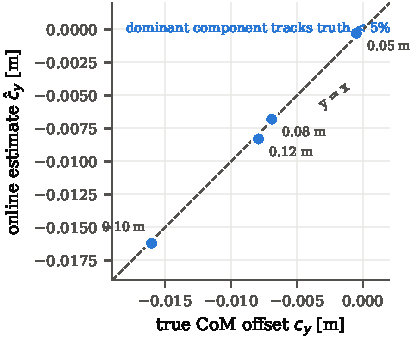
\includegraphics[width=\linewidth]{figs/fig4_cxy_vs_truth.pdf}
\caption{Online CoM-offset estimate vs.\ ground truth across an eccentricity sweep. The
dominant ($c_y$) component tracks truth to $<5\%$ with no attachment measurement---the
estimate uses only motor-speed-reconstructed torques.}
\label{fig:cxy}
\end{figure} \emph{Highlight:} on the hardest cell (\SI{0.3}{kg}/\SI{0.10}{m}) the
truth version diverges 2/5 while the online version is stable 0/5---the divergent truth runs
apply an off-nominal deep grasp instantaneously at full geometry (hover roll torque
\SI{0.459}{N.m} $= \SI{92}{\percent}$ of $\tau_{\max}$), whereas the online version ramps from
a prior. A later paired A/B reproduces this independently (truth $1/8$ vs.\ online $0/8$; the
divergent run was again an outlier grasp at \SI{82}{\percent} of $\tau_{\max}$, while an online
run in the same cell grasped \emph{further} off-centre at \SI{84}{\percent} and completed),
pooling to truth $3/13$ vs.\ online $0/13$.

\emph{Geometry--mass decoupling ablation.} Low stress: decoupled 15/15 no droop vs.\ coupled
10/15 (droop rate $33\% \to 0\%$)---the reproducible evidence for decoupling. We also probed a
high-stress regime ($m_{\min}=1.0$, allowing the mass estimate room to collapse toward the
lower bound) with per-run manifests ($n=16$ per group): here \emph{both} paths were stable
($0/16$ divergence each), and the coupled estimate never actually probed the collapse regime
(minimum $\hat m = 2.03$, all runs converging near truth). An earlier un-logged observation of
coupled-path divergence traced to \emph{off-nominal deep grasps} (attachment depth outliers
near the torque-saturation boundary), an attach-depth artifact rather than a systematic
coupled-vs-decoupled effect at nominal conditions; we therefore rest the ablation on the
low-stress droop result and the bootstrap-decoupling mechanism, not on a divergence-rate
difference.

\fi

\begin{figure}[tb]
\centering
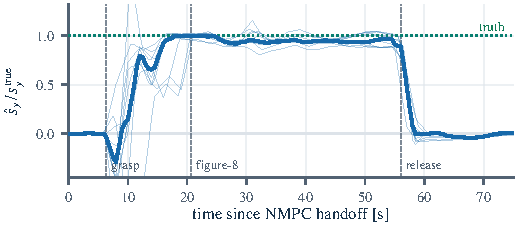
\includegraphics[width=\linewidth]{figs/fig_moment_truth.pdf}
\caption{First mass moment against ground truth (\SI{0.15}{kg} at \SI{2}{m/s}, $n=11$, each
normalised by its own truth).
Truth is reconstructed offline as $m_P r_y$ from the simulator-measured grasp offset and never
reaches the estimator, which runs with no horizontal attachment geometry. $\hat{s}_y$ is zero
before grasp, rises with no attach notification, holds near truth through the figure-eight,
and decays to zero after release. Across the original campaign's 31 eligible flights the carry-phase estimate
is biased toward zero (slope 0.85; median magnitude underestimate 10.8\%, same direction in
31/31; largest at \SI{0.30}{kg}, median 15.7\%). The cause of this bias is not identified; the
moment-gated detector uses the ratio $\|s\|/\|s\|_{\mathrm{ref}}$, which is insensitive to a
common scale bias.}
\label{fig:moment}
\end{figure}

% Focused system-level validation for the eventless interface.
% The complete detector-development record remains in sec_autonomous_release.tex.
\subsection{Eventless grasp--release lifecycle}\label{sec:autorelease}

\begin{figure*}[t]
\centering
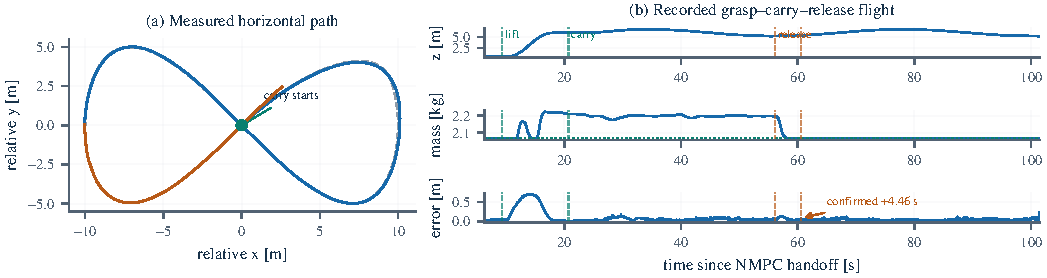
\includegraphics[width=0.95\textwidth]{figs/fig_mission.pdf}
\caption{One eventless flight from the final batch (\SI{0.15}{kg}, \SI{2}{m/s}).
Left: the measured horizontal path (blue while carrying, orange after release)
against the nominal reference including its amplitude ramp (grey dashed).
Right: recorded height, controller-consumed mass estimate, and position-error norm
through grasp, lift, carrying, release command, and confirmation.
This flight confirms in maneuver, 4.46 s after the command; it illustrates one
execution and does not replace the cohort statistics in Table~\ref{tab:complete}.}
\label{fig:mission}
\end{figure*}

The controller issues the gripper-release command itself, but deliberately does not use that
command to clear its payload model: a commanded release is not proof of physical detachment.
The proposed interface consumes only healthy, fresh $m/s/J$ frames and completes a release only
after its no-payload confidence remains above 0.90 for \SI{1.0}{s}. We report every eventless
flight in the final campaign that met the pre-registered eligibility criteria: successful MHE
payload evidence and survival to the release command. Exclusions are reported below and are not
absorbed into the completion result.

\paragraph{Paired external-event baseline}
We retain the pre-registered paired ablation rather than selecting arm~B alone after the
comparison. Arm~A is an external-event baseline: it treats the release command as the
detachment event and immediately resets payload geometry and inner-loop scaling. Arm~B is the
proposed eventless interface above. A pair enters this comparison only when both arms satisfy
the same eligibility criteria. There are 23 such pairs (8/7/8 across the three conditions); both arms complete
23/23 releases with no observed post-release instability (Table~\ref{tab:paired-event}).
Arm~A has zero confirmation delay by definition, whereas arm~B waits for physical evidence.
This comparison therefore quantifies the cost of refusing the event shortcut; it is not
evidence that arm~A detects physical detachment.

\begin{table}[tb]
\caption{Paired external-event ablation. Arm~A clears the model from the command by
construction; arm~B requires estimator evidence. The last row injects a command/physical-
detachment mismatch; ``early'' means model clearing before the DetachableJoint is removed.
The one valid but unpaired arm~B run of that row also did not clear early (0/6).}
\label{tab:paired-event}
\centering
\scriptsize
\setlength{\tabcolsep}{2.5pt}
\begin{tabular}{@{}lcccc@{}}
\toprule
condition & pairs & A compl. & B compl. & early clear A/B \\
\midrule
\SI{0.15}{kg}, \SI{4}{m/s} & 8 & 8/8 & 8/8 & -- \\
\SI{0.30}{kg}, \SI{4}{m/s} & 7 & 7/7 & 7/7 & -- \\
\SI{0.15}{kg}, \SI{2}{m/s} & 8 & 8/8 & 8/8 & -- \\
\midrule
nominal pooled & 23 & 23/23 & 23/23 & -- \\
\SI{0.15}{kg}, \SI{2}{m/s} + \SI{4}{s} hold & 5 & 5/5 & 5/5 & 5/5 / 0/5 \\
\bottomrule
\end{tabular}
\end{table}

To exercise the mismatch that motivates the paper, a fault injector received the normal
release command but retained the physical DetachableJoint for a median \SI{4.01}{s}. Twelve
arm-runs were attempted; one arm~A run never armed PX4, leaving five valid pairs and one
valid but unpaired arm~B run. In all five pairs arm~A cleared its payload model at the
command---a median \SI{4.01}{s} before physical detachment. Arm~B never cleared before
detachment in any of its six valid runs, the unpaired one included: it entered
\textsc{unresolved} in 5/6 and then confirmed a median \SI{12.45}{s} after detachment, while
the remaining run confirmed \SI{3.00}{s} after detachment without entering
\textsc{unresolved}. Within the five pairs, median position-error peaks during the
four-second hold were \SI{0.071}{m} (A) and \SI{0.068}{m} (B), so we claim a semantic safety
distinction, not a tracking advantage. All eleven valid runs had an independent Gazebo
\texttt{DETACHED} state record.

The eventless interface completed autonomous release confirmation in 31/31 eligible flights with no
observed post-release instability (Table~\ref{tab:complete}). The two-sided \SI{95}{\percent}
Clopper--Pearson interval is $[\SI{88.8}{\percent},\SI{100}{\percent}]$, so this result
demonstrates closed-loop feasibility rather than a zero failure rate.

The confirmation delay is \emph{bimodal}, and the two modes are two distinct control paths
rather than a spread within one path. In \SI{42}{\percent} of flights the no-payload
confidence crosses threshold while the vehicle is still flying the figure-eight and
confirmation completes in \SI{3.46}{s} (median; one such flight is shown in
Fig.~\ref{fig:mission}). In the remaining \SI{58}{\percent} no moment vote is available in maneuver---$\hat s$
has drifted under sustained excitation or the frozen reference never formed---so the system
reaches its \SI{12}{s} timeout, declares the payload
state \textsc{unresolved}, and executes a \SI{3}{s} smooth brake to hover; deceleration
alone restores observability and confirmation then completes at \SI{16.48}{s} (median).
Reporting one median across both paths would be misleading, so Table~\ref{tab:complete}
separates them.

In 26 of the 31 flights the payload-presence machine made exactly two transitions---one
load declaration at grasp and one empty declaration at release---with no spurious
carrying-phase transition. In the five remaining flights, all of which confirmed
in maneuver, the estimator's presence machine never declared \textsc{empty} within the logged
window (over \SI{40}{s} past confirmation); confirmation rested on the published no-payload
confidence alone, as detailed below. Four of the 31 load declarations were
raised by the estimator's own directional thrust-residual evidence rather than by sustained mass
evidence; no external grasp signal was consumed. The published first
moment decayed continuously rather than stepping to zero (Fig.~\ref{fig:moment}), confirming that recovery used the
intended estimator interface rather than the controller's release command.

\begin{table}[tb]
\caption{Eventless release completion and confirmation delay (all eligible eventless flights). Delay runs
from the release command to the frame where the no-payload confidence has held for the full
\SI{1.0}{s}, so it includes that hold. The two delay columns are distinct control paths and
must not be pooled.}
\label{tab:complete}
\centering
\scriptsize
\setlength{\tabcolsep}{3.5pt}
\begin{tabular}{@{}lcccc@{}}
\toprule
 & & & \multicolumn{2}{c}{delay median [IQR]} \\
\cmidrule(lr){4-5}
condition & $n$ & compl. & in-maneuver & via brake-to-hover \\
\midrule
\SI{0.15}{kg}, \SI{4}{m/s} & 9 & 9/9 & \SI{2.78}{s} [2.76, 2.90] & \SI{16.56}{s} [16.46, 16.60] \\
\SI{0.30}{kg}, \SI{4}{m/s} & 11 & 11/11 & \SI{7.08}{s} [6.96, 7.50] & \SI{16.40}{s} [15.76, 16.60] \\
\SI{0.15}{kg}, \SI{2}{m/s} & 11 & 11/11 & \SI{3.46}{s} [3.16, 4.36] & \SI{16.48}{s} [16.40, 16.50] \\
\midrule
pooled & 31 & 31/31 & \SI{3.46}{s} [2.86, 4.46] & \SI{16.48}{s} [16.36, 16.60] \\
\bottomrule
\end{tabular}
\\[2pt]
\footnotesize Pooled completion \SI{100}{\percent}, two-sided \SI{95}{\percent}
Clopper--Pearson CI $[\SI{88.8}{\percent}, \SI{100}{\percent}]$; overall delay max
\SI{16.70}{s}. The share of flights confirming only after the brake-to-hover maneuver is
\SI{56}{\percent}, \SI{64}{\percent} and \SI{55}{\percent} (rows in order) and
\SI{58}{\percent} pooled; the complement confirms in maneuver.
\end{table}

\paragraph{Safety boundary}
The 31/31 batch validates the interface once its release evidence is accepted; it does not
validate a universally robust detector. We therefore tested three physically distinct evidence
sources: payload quantity, directional thrust residual, and collapse of the normalized first
moment. A fast branch combining quantity and residual without moment evidence declared release
prematurely in 3/9 randomized flights during a \SI{4}{m/s} figure-eight. Loaded-flight mass
estimates could remain below the nominal empty threshold for up to \SI{48}{s}, while a dynamic
thrust excursion reached \SI{-1.69}{N}, exceeding the \SI{-1.47}{N} weight change of the
smallest payload. Neither source is therefore reliable on its own in this regime.

We rejected that branch: the estimator's unified release detector now fires only on fresh,
successful moment-collapse evidence (the slow and moment--residual paths); the legacy
mass-domain route that remains is quantified below. Ambiguous cases enter \textsc{unresolved};
a timeout does not clear the model or reset adaptive state. In a subsequent 12-flight
randomized validation, no flight declared release before the command: all 11 confirmed
releases passed through moment-gated paths (9 moment--residual, 2 slow) with a median detector
delay of \SI{1.9}{s}, and one remained safely unresolved. That validation preceded the frozen
moment reference.

\paragraph{Release paths in the final batch}
The moment-gated detector is not the only route to confirmation in the final code, and the
31-flight batch of Table~\ref{tab:complete} exercised three. The controller confirms release
when the published no-payload confidence---the product of mass, first-moment and inertia
``empty'' scores, where the moment score uses an absolute bound on $\lVert s\rVert$ rather than
the frozen-reference ratio---holds above 0.90 for \SI{1.0}{s} on healthy, fresh frames.
(i)~In 19/31 flights (9/9, 1/11 and 9/11 in the rows of Table~\ref{tab:complete}) the
moment-gated detector declared release first and the confidence followed. (ii)~In 7/31
flights, all at \SI{0.30}{kg}, the flights that reached
\textsc{unresolved}, the frozen moment reference was never established because its
low-dynamic, in-envelope sampling window never filled, so the ratio test never ran; the
confidence crossed threshold during or shortly after the brake to hover, and the estimator's
mass-domain path ($m_P<\SI{0.030}{kg}$ for 20 frames, counted only in low-dynamic flight)
declared release 0.9--\SI{3.1}{s} later. (iii)~In 5/31 flights (three at \SI{0.30}{kg}, two at \SI{2}{m/s}), all
confirmed in maneuver, the reference was likewise never established and the estimator never
declared release; confirmation rested on the confidence alone. No flight in any path declared
release before the command. The supported safety conclusion is therefore bounded: the randomized validation
supports the moment-gated detector, while the final batch shows that 12/31 confirmations did
not pass through it. Broader detector robustness remains outside the present claim.


The cohort is conditional on successful MHE payload evidence and survival to the release
command. Of 40 eventless flights, 31 were eligible: six crashed before release and three lacked
MHE payload evidence. The available logs cannot distinguish physical capture failure from
estimator non-recognition in those three cases. Confirmation delay is a median \SI{3.46}{s}
when it clears in maneuver and \SI{16.48}{s} when the vehicle must first brake to hover.

Across the paired campaign there were 81 attempts: arm~A contributed 41 attempts (30 eligible,
11 pre-release crashes), and arm~B contributed 40 (31 eligible, six pre-release crashes and
three payload-evidence failures). Only the 23 pairs in which both arms were eligible enter
Table~\ref{tab:paired-event}; all 31 eligible B flights enter Table~\ref{tab:complete}. These
are different estimands and are not substituted for one another. Tail-window tracking is not
compared: arm~B brakes to hover after an unresolved timeout, while arm~A continues the
figure-eight.


\iffalse
\subsection{Legacy full-flow visualization}
Figure~\ref{fig:b5} is retained as a qualitative visualization of the physical
grasp--carry--release sequence. It was recorded before the final continuous $m/s/J$ interface
and therefore does not carry the eventless-interface claim of
Sec.~\ref{sec:autorelease}. In that legacy run, a figure-eight carrying an eccentric
\SI{0.3}{kg} load achieved \SIrange{1}{3}{cm} loaded tracking, a release-transient peak of
\SI{0.21}{m}, ${\sim}\SI{2.5}{s}$ recovery, and zero divergence.

\begin{figure}[tb]
\centering
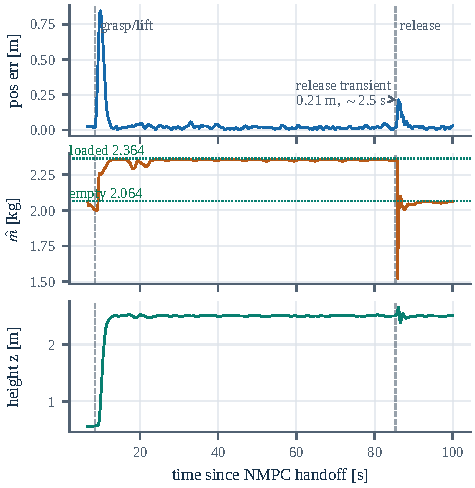
\includegraphics[width=\linewidth]{figs/fig5_b5_fullflow.pdf}
\caption{Legacy complete grasp $\rightarrow$ carry $\rightarrow$ release visualization
(dense $10$\,Hz telemetry throughout). The mass estimate tracks \emph{both} transitions---rising to the
loaded value ($2.364$~kg) at grasp and returning to empty ($2.064$~kg) at release---and the
release transient (position-error peak $0.21$~m, ${\sim}2.5$~s recovery) is fully captured.
This run predates and does not validate the final eventless $m/s/J$ interface; that claim uses
the eventless cohort in Sec.~\ref{sec:autorelease}.}
\label{fig:b5}
\end{figure}
\fi

\subsection{Baselines and ablations}
\textbf{L1-NMPC three-way matrix (Table~\ref{tab:matrix}).} \{truth, online, l1\} $\times$
\{0.2, 0.3\}~kg $\times$ \{0.05, 0.10\}~m, $n=5$, 60/60 runs stable, zero divergence. (i)
Within-cell transient peaks agree to \SI{0.05}{m}; L1 is higher in the two low-eccentricity
cells ($p=.008$, $.012$ uncorrected, not surviving correction over eight tests), so we claim
\emph{no} transient advantage. (ii) Against the deployed \emph{online} estimate, \textbf{L1 recovers
\SIrange{8}{32}{\percent} slower} (median \SI{16}{\percent}; significant in three of four
cells); the mechanism is that its compensation low-pass cutoff
$\omega_c$ is bounded by closed-loop stability (0.5 stable, 1.0 unstable on this platform), a
bandwidth wall that explicit estimation does not face. (iii) L1 yields no interpretable
$m$/$c_{xy}$ and still requires the same class prior for gain scaling; it is a translational
3-DoF augmentation driven by $T_{\text{phys}}$ (the commanded thrust self-excites). The larger
\emph{truth} peak in cell 0.3/0.10 is not explained; more accurate parameters need not reduce a
transient peak. All three arms used the earlier mass-only MHE.

\begin{table}[tb]
\caption{Three-way method $\times$ scenario matrix ($n=5$): pos\_err peak~[m] / recovery~[s].}
\label{tab:matrix}
\centering
\begin{tabular}{@{}lccc@{}}
\toprule
cell (mass/ecc) & truth & online & l1 \\
\midrule
0.2 / 0.05 & 0.806 / 4.28 & 0.768 / 3.70 & 0.821 / 4.26 \\
0.2 / 0.10 & 0.794 / 3.62 & 0.810 / 3.92 & 0.812 / 4.24 \\
0.3 / 0.05 & 0.834 / 3.56 & 0.837 / 3.72 & 0.883 / 4.90 \\
0.3 / 0.10 & 1.011 / 3.64 & 0.876 / 3.88 & 0.891 / 4.54 \\
\bottomrule
\end{tabular}
\end{table}

\section{Limitations and Future Work}\label{sec:limits}
All system-level evidence is presently SITL-only. Hardware migration replaces simulated motor
speeds with ESC telemetry and must re-identify thrust/torque coefficients, noise floors, timing,
and gripper compliance before free flight.

\emph{Thrust proxy.} In simulation the plant uses the same square law $k\omega^2$ as the
estimator, and motor speeds are exact. Scaling only the estimator's thrust map by
\SI{\pm5}{\percent} (\SI{0.15}{kg}, \SI{2}{m/s}, four flights each) caused no pre-command release
but defeated the interface in both directions: at 0.95 the payload was never recognized (4/4),
and at 1.05 a phantom \SI{0.09}{kg} persisted after release (3/4 \textsc{unresolved}). Thus $k$
must be calibrated well within \SI{5}{\percent}; speed noise, delay and induced inflow
\cite{bangura2012} remain untested.

\emph{Missing baselines.} We have not compared against a fixed-parameter NMPC, a CUSUM detector
\cite{basseville1993} on the same signals under a matched false-alarm constraint, or L1-NMPC with
the final estimator. The vertical arm $r_z$ is unobservable from the
thrust-moment channel and remains a weak prior; the $s_x$/pitch channel is noisier than
$s_y$/roll. The deployed diagonal inertia approximation also drops the small
$O(r_{xy}^{2})$ and yaw-inertia terms.

\emph{Release-detector boundary.} First-moment augmentation is now part of the default path.
\iffalse
and the 21/21 paired result demonstrates that its output can drive the complete NMPC recovery
without a drop event. It does not establish detector robustness: historical replay still misses
14/72 releases, and the 95\% interval from 21 successes permits a true failure rate near
16\%. The key structural issue in the audited profile was that its shared \SI{4.4}{N} residual
threshold was chosen to suppress the residual path for a \SI{0.30}{kg} envelope study, but the smallest supported
\SI{0.15}{kg} payload produces only a \SI{1.47}{N} weight step. Lowering that shared threshold
would also change MHE weight scheduling and would confound earlier ablations. The subsequent
release-only detector solved that coupling but its fastA branch failed the randomized smoke:
3/9 flights released the estimator state prematurely. In loaded figure-eight flight, payload
mass had a fifth percentile of \SI{-0.1032}{kg} relative to the bare airframe and remained below
the nominal empty threshold for a median \SI{14}{s} (maximum \SI{48}{s}); quantity is therefore
not valid evidence in that regime. Adding a lower-bound exclusion still leaves 13.6\% of loaded
frames below threshold, while a weak moment gate has not been distributionally justified.
We consequently reject fastA and retain only moment-gated paths. If they time out, the controller
must enter a conservative hover/land abort while keeping the payload state unresolved; timeout
must not clear the model or reset adaptive state. This accepts a possible missed release under
the synthetic $\rho=1.52$ cross-boundary stress case rather than retaining a path with an
observed one-third flight-level false-release rate. A post-removal replay flagged one apparent
slow-path false release in run~152924, but that record is not a valid clean counterfactual: it was
generated after the old fastA branch had already cleared and re-armed the online lifecycle.
Nevertheless, it exposes a real upstream defect. Five consecutive MHE failures triggered a
re-anchor that explicitly set $\hat s=0$, and the release counters consumed that invalid value
before a fresh successful solve. The appropriate correction is health/freshness gating and
counter reset on solve failure or re-anchor, not a post-hoc lower ratio cutoff. This correction
was then exercised in 12 clean online flights: none released before the command, 11/12 obtained
valid late evidence (median detector delay \SI{1.9}{s}), and the remaining flight stayed unresolved
without clearing the model. Three flights crossed the \SI{12}{s} unresolved timeout and two later
recovered when delayed evidence arrived.

A coverage gap in that smoke was subsequently corrected: the unified detector had remained
nested under a legacy mass-arm latch, so one autonomously detected attachment never entered the
moment decision. Commit \texttt{ddfe9d2} moved the unified detector under the autonomous load
latch plus health while leaving the mass-arm local to the legacy mass-only branch. The first four
post-fix flights then exposed a different pre-existing issue and were stopped before acceptance:
the running maximum used as the loaded-moment reference absorbs figure-eight estimation errors.
Samples beyond the simulation envelope $m_{p,\max}r_{xy,\max}=\SI{0.039}{kg.m}$ occur in both the
old data (49/644 frames, 7.6\%, four of 11 flights) and the post-fix data (49/268, 18.3\%, three of four
flights), beginning about \SIrange{26}{28}{s} after attachment in the dynamic segment. Thus the
gate change increased exposure but did not create the estimator error. A safe revision must build
a robust loaded-moment reference from an autonomously identified low-dynamic, healthy,
in-envelope window, freeze it before dynamic flight, and treat out-of-envelope samples as invalid
evidence and an estimator-quality diagnostic. Raw $\hat s$ may also fail to return to zero after a
real drop; this remains a safe miss handled by \textsc{unresolved}, not permission to clear $s$
from the controller's command.
\fi
The development-stage tests and the three final-batch confirmation paths are reported in
Sec.~\ref{sec:autorelease}; 32/36 completions do not establish distribution-wide detector
robustness. In 13 of the 32 completed flights the healthy, low-dynamic, in-envelope reference
window never filled after the \textsc{loaded} declaration, so the moment-ratio test never ran.
Out-of-envelope $\hat s$ samples are excluded from moment votes but still reach the
controller's $c_{xy}$ through filtering and slew limits. The envelope assumed a
\SI{0.13}{m} grasp offset while the gripper admitted \SI{0.15}{m}; this affected 2 of 13
\SI{0.30}{kg} flights and does not explain most missing references. Reliable reference formation
therefore remains necessary for a robust autonomous release detector.

All reported release batches explicitly enable the release-evidence path. Its built-in
default is off, under which every flight ends \textsc{unresolved}, so deployment requires an
explicit enable plus startup validation of the configuration.

\emph{First-moment drift.} Sustained figure-eight excitation can increase
$\lVert\hat s\rVert$ from \SI{0.012}{\kilo\gram\metre} to
\SI{0.031}{\kilo\gram\metre}; withholding moment evidence then delays confirmation.
Deceleration restored the vote within \SIrange{3.3}{3.4}{s} in the affected test flights.
Together with missing-reference cases, this yields the brake-to-hover delays in
Table~\ref{tab:complete}. An online counter of first-moment envelope exceedances correlates
with this outcome at \SI{4}{m/s} (in-maneuver confirmation 9/10 for zero exceedances
versus 2/10 otherwise; Fisher $p=0.006$), but misses all six delayed \SI{2}{m/s} cases.
Earlier exit from the maneuver remains unimplemented
and requires validation.

\emph{Operating limit.} \SI{0.30}{kg} at \SI{4}{m/s} is a stress test at the vehicle's actuator
limit, not an operating point. Hover needs \SI{74}{\percent} of maximum thrust, but torque binds:
in the figure-eight, pitch torque saturated within \SI{98}{\percent} of 5-s diagnostic windows
and yaw within \SI{53}{\percent} (\SI{46}{\percent}/\SI{16}{\percent} at \SI{0.15}{kg},
$\le\SI{6}{\percent}$ at \SI{2}{m/s}), and body-rate scaling ran at a median 4.39 of its 5.0 cap. Three of the five arm~B
pre-release crashes (figure-eight divergences) and three of the four incomplete releases occurred
there, and the legacy arm~A crashed during or just after lift in 11 of 16 attempts because its
rate scaling starts from the lower-bound mass estimate while the box is still grounded. Every
eligible \SI{2}{m/s} flight confirmed release. We claim safe release semantics, not reliable
flight, at this limit; deployment needs torque margin.

\emph{Estimator failures.} In four flights the published mass never left the empty value (in two,
repeated solver failures re-initialized from a lower-bound seed); the three at \SI{4}{m/s} flew
without diverging and stayed \textsc{unresolved}. In one \SI{0.30}{kg} flight the estimate was
unhealthy for \SI{48}{s} before release; because the phase-timed release command is not gated on
estimator health, the frozen model no longer matched the vehicle after detachment and it diverged.
A window vertical-force balance now seeds re-initialization (pre-registered A/B at this
condition: figure-eight re-initializations 29 to 1); the reported cohort predates it, and
health-gated release remains open.

A sustained vertical up/downdraft remains intrinsically confounded with a payload change on a
collective-thrust-only residual; wind is not evaluated in the reported cohort.

\emph{Simulator fidelity.} (i) gz-sim Harmonic cannot change a link's inertia at runtime in a
way the physics adopts (issue \#2733), so every payload change is produced by the
DetachableJoint platform, which attaches a separate rigid body (\S\ref{sec:sim}). (ii) The payload is rigidly attached; gripper compliance and pendulum modes
are not modeled. Neither affects which signals the estimator consumes.

\section{Conclusion}
We presented an eventless payload-model interface for quadrotor NMPC that estimates composite
mass and the horizontal first mass moment from odometry and a rotor-speed thrust proxy, and
that clears its payload model only on persistent estimator evidence, never on its own release
command. In PX4 SITL the complete interface confirmed release in 32 of 36 eligible flights through
three confirmation paths, with median delays of \SI{3.46}{s} in maneuver and \SI{16.56}{s} after
braking to hover; all four failures arose from estimator failure at \SI{4}{m/s}, three of them
at the vehicle's torque limit. Under a \SI{4}{s} delayed detachment, persistent confirmation, with or without the
command, avoided the early model clearing of a command-triggered baseline (5/5); the eventless
interface additionally detected 10 of 18 unsignaled payload losses that a command-armed
confirmer cannot see. Hardware validation, thrust-map mismatch, reliable moment-reference formation, gating release
on estimator health, and stronger baselines remain open.

\bibliographystyle{IEEEtran}
\bibliography{refs}

\end{document}
